% SIDe 2026 submission — IEEE double-column conference template.
% ANONYMITY: set \blindtrue below for a double-blind submission and the author
% block collapses to one anonymous line. It is currently \blindfalse, so names,
% affiliations, ORCIDs and emails appear. The Reproducibility section still
% promises an anonymised repository link; the named branch carries the real
% URL, so switching to \blindtrue swaps it back out for that promise.
%
% Reference audit, 6 Sep 2026: [5] Boujmiraz, [12] Schwerter and [18] Phiri
% were each verified against Crossref/arXiv/DataCite and are correct as cited.
% Build:  latexmk -pdf main.tex     (or upload this folder to Overleaf)
% Needs:  IEEEtran.cls (bundled with TeX Live/MiKTeX and available on Overleaf)
%         figures/fig1_explanation_instability.pdf

\documentclass[conference]{IEEEtran}
\IEEEoverridecommandlockouts

\usepackage{cite}
\usepackage{amsmath,amssymb}
\usepackage{graphicx}
\usepackage{booktabs}
\usepackage{url}
\usepackage[T1]{fontenc}
\usepackage[utf8]{inputenc}
\usepackage{textcomp}
\usepackage{xcolor}
% Loaded last, as hyperref requires. Without it \url only sets the address in
% typewriter type; the link is not clickable. hidelinks keeps IEEE's plain look.
\usepackage[hidelinks,breaklinks]{hyperref}

\graphicspath{{figures/}}

% IEEEtran wants no page numbers in the submitted PDF.
\pagestyle{empty}

% IEEEtran puts all \and-separated authors in one row, which overflows at six.
% \linebreakand closes the current row and opens the next one.
\makeatletter
\newcommand{\linebreakand}{%
  \end{@IEEEauthorhalign}\hfill\mbox{}\par\mbox{}\hfill\begin{@IEEEauthorhalign}}
\makeatother

\newif\ifblind
\blindfalse  % \blindtrue for anonymous review

\begin{document}

\title{A Five-Institution Benchmark for Student-Risk Models, and the Reference Points Explanation-Stability Claims Need}

\ifblind
\author{\IEEEauthorblockN{Anonymous submission}}
\else
\author{
\IEEEauthorblockN{A. S. Talgatov}
\IEEEauthorblockA{\textit{Master degree student} \\
\textit{School of Software Engineering} \\
\textit{Astana IT University} \\
Astana, Kazakhstan \\
ORCID: 0009-0006-3463-4644 \\
a1byn.talgat05@gmail.com}
\and
\IEEEauthorblockN{S. A. Nurgaliyeva*}
\IEEEauthorblockA{\textit{PhD in computer science} \\
\textit{School of Software Engineering} \\
\textit{Astana IT University} \\
Astana, Kazakhstan \\
ORCID: 0009-0009-5880-6166 \\
symbat.nurgaliyeva@astanait.edu.kz}
\and
\IEEEauthorblockN{Z. Basheyeva}
\IEEEauthorblockA{\textit{School of Software Engineering} \\
\textit{Astana IT University} \\
Astana, Kazakhstan \\
ORCID: 0000-0001-9605-2101 \\
zhuldyz.basheyeva@astanait.edu.kz}
\linebreakand
\IEEEauthorblockN{A. Sakhipov}
\IEEEauthorblockA{\textit{PhD, Assistant Professor} \\
\textit{IEEE Senior Member} \\
\textit{School of Software Engineering} \\
\textit{Astana IT University} \\
Astana, Kazakhstan \\
ORCID: 0000-0003-1045-4199 \\
aivar.sakhipov@astanait.edu.kz}
\and
\IEEEauthorblockN{N. Turysbek}
\IEEEauthorblockA{\textit{School of Cybersecurity} \\
\textit{Astana IT University} \\
Astana, Kazakhstan \\
ORCID: 0009-0000-0932-3525 \\
n.turysbek@astanait.edu.kz}
\and
\IEEEauthorblockN{M. Kali}
\IEEEauthorblockA{\textit{School of Cybersecurity} \\
\textit{Astana IT University} \\
Astana, Kazakhstan \\
ORCID: 0000-0001-5588-8164 \\
marzhan.kali@astanait.edu.kz}
}
\fi

\maketitle
\thispagestyle{empty}

\begin{abstract}
Studies of student-risk models are almost always run on one dataset, and studies
of their explanations on one importance estimator. We release a benchmark that
removes the first restriction and use it to show why the second one matters. The
benchmark covers 63 cohorts from five universities on five learning-management
platforms in four countries, 35{,}529 distinct students, harmonised to one
seven-feature schema, with adapters and frozen results released. Three findings
follow. First, predictability varies far more than any single-dataset study can see, and most of that variation tracks the institution rather than the task: within-cohort ROC-AUC spans 0.384 to 0.953 across the 63 cohorts and 0.527 to 0.845 across institution means, and 18 cohorts have bootstrap intervals covering chance, so a single-dataset result describes its dataset.
Second, we test on this population the reported finding that the choice of explainer matters more than the sample a model is trained on, and find the comparison has no estimator-free answer. Permutation importance and SHAP agree with each other at Kendall $\tau$ 0.410, which is above permutation's own within-cohort reference of 0.345 and below SHAP's of 0.592: the reported ordering holds under one estimator and reverses under the other. Establishing that required reference points the original design could not supply --- a noise floor of 0.706, a within-cohort reference measured under each estimator, and an analytic random baseline. Third, a single-estimator stability study reports a conclusion conditional on an undeclared choice: measuring how much a year of retraining costs a feature ranking gives $\tau$ 0.256 under permutation importance and 0.508 under SHAP, while the cost itself is the same under both, 0.089 and 0.083, so the estimator moves the reported level by three times the effect under study. We also report two
measurement hazards found by auditing our own pipeline, and a zero-training
baseline that gradient boosting fails to beat in 38 of 63 cohorts.
\end{abstract}

\begin{IEEEkeywords}
benchmark, learning analytics, explainable AI, feature importance, replication,
trustworthy AI
\end{IEEEkeywords}

\section{Introduction}

Two habits shape the empirical literature on student-risk prediction. Models are
developed and evaluated on a single dataset, usually one institution's.
Explanations are computed with a single importance estimator, usually whichever
library the authors reached for. Neither habit is examined, because examining
either requires resources most studies do not have: many institutions, or many
estimators applied to the same models.

This paper supplies both and reports what they show. It is a resource paper with a measurement result attached, not a methods paper: we propose no new model, explainer or transfer technique. Three of our own candidate methods were discarded when controls showed they did not beat far simpler alternatives; those controls are in Section~\ref{sec:controls} because they bound how the rest should be read.

Contributions:

\begin{enumerate}
\item A public five-institution benchmark: 63 cohorts, 35{,}529 distinct
students, five platforms, four countries, one harmonised schema, with adapters,
cohort definitions and frozen results released (Section~\ref{sec:data}).
\item The spread of predictability across institutions, which a single-dataset
study cannot observe (Section~\ref{sec:pred}).
\item An attempted replication of the finding that explainer choice matters more than the training sample \cite{swamy2022}, on a population five times larger and structurally different, which turns out to depend on which estimator supplies the reference (Section~\ref{sec:agree}).
\item A methodological consequence: single-estimator stability studies report
conclusions conditional on an undeclared choice, and we quantify by how much
(Section~\ref{sec:cond}).
\item Two measurement hazards and a baseline audit that changed our own
conclusions mid-project (Section~\ref{sec:controls}).
\end{enumerate}

\section{Related Work}

\textbf{Prediction on public LMS data.} Gradient boosting or random forests over
weekly activity features, with post-hoc explanations attached, is the standard
configuration, and reviews catalogue hundreds of such systems
\cite{bettahi2025,boujmiraz2026,guevara2025}. The reporting unit is one
configuration on one cohort.

\textbf{Cross-institution work.} Transfer of student models is well studied: across 24 Moodle courses \cite{lopez2020,lopez2022}, four US universities on private data \cite{gardner2023}, two universities \cite{schwerter2026}, 532 courses at one institution \cite{riestra2021}, and between partner institutions as early as 2014 \cite{jayaprakash2014}. What is missing is not the question but a harmonised, multi-platform corpus another group can run against. That is the gap this benchmark fills.

\textbf{Explanation stability.} Tiukhova et al.\ showed with SHAP that importance
rankings of student-success models shift across cohorts and years of one
programme \cite{tiukhova2024}. Swamy et al.\ compared five explainers on
bidirectional LSTM models over five MOOCs and concluded that ``the choice of
explainer is an important decision and is in fact paramount to the interpretation
of the predictive results, even more so than the course the model is trained on''
\cite{swamy2022}. Theirs is the conclusion we set out to replicate. We claim no priority for it, and where we fail to reproduce it we report that as a result about measurement rather than as a refutation of their setting, which differs from ours in model family, features and population. Their design established the ordering
structurally --- principal-component scatter and per-course heatmaps --- but
could not put the two sources of variation on a common numeric scale, because
their importance vectors have course-specific lengths. A harmonised schema
removes that obstacle, which is the extension we contribute. Outside education,
Hooker et al.\ show permutation importance evaluates a model off its own data
manifold and argue a defensible estimate requires refitting \cite{hooker2021};
Krishna et al.\ document disagreement between explanation methods generally
\cite{krishna2022}; and Verdinelli and Wasserman prove that SHAP and
leave-one-covariate-out target genuinely different estimands
\cite{verdinelli2024}, which we treat as the correct interpretation of part of
our result rather than as a competing explanation of it.

\section{The Benchmark}\label{sec:data}

\subsection{Five institutions, five platforms}

Table~\ref{tab:cohorts} summarises the corpus. A cohort is one course, one
academic period, one institution, admitted with at least 50 students and at least
15 in the rarer outcome class. Cohort sizes sum to 45{,}158, but only 35{,}529
students are distinct: 7{,}995 of them, 22.5\,\%, appear in more than one cohort, which
Section~\ref{sec:controls} shows is not a bookkeeping detail. Outcome definitions
differ across institutions and are perfectly collinear with institution, so no
analysis here separates a label effect from an institution effect; OULAD in
particular counts withdrawal as failure, which a clickstream predicts almost by
construction.

% Spans both columns: five columns of text do not fit a 3.5 in column, and at
% in-column width the institution names collide with the adjacent body text.
\begin{table*}[t]
\caption{The benchmark, and within-cohort discrimination per institution. Pass rate is the share of a cohort's students recorded as passing, shown as the range over that institution's cohorts; the AUC column is the mean over them. Within-cohort ROC-AUC is 5-fold cross-validated gradient boosting on the shared seven-feature schema.}
\label{tab:cohorts}
\centering
\begin{tabular}{@{}llccrrr@{}}
\toprule
Institution & Platform & Country & Cohorts & Students & Pass rate & Within-cohort AUC \\
\midrule
Open University \cite{kuzilek2017}       & OU VLE & UK           & 19 & 30{,}059 & 0.34--0.73 & 0.845 \\
Univ.\ of KwaZulu-Natal \cite{raghavjee2026} & Moodle & South Africa & 16 & 7{,}254  & 0.60--0.95 & 0.667 \\
KU Leuven \cite{tiukhova2026}            & Toledo & Belgium      & 6  & 3{,}939  & 0.51--0.75 & 0.608 \\
Univ.\ de Oviedo \cite{riestra2021}      & Moodle & Spain        & 20 & 3{,}789  & 0.26--0.84 & 0.606 \\
Univ.\ of Zambia \cite{phiri2026,phiri2026paper} & Moodle & Zambia       & 2  & 117      & 0.25--0.38 & 0.527 \\
\midrule
Total & 5 platforms & 4 countries & 63 & 35{,}529 distinct & 0.25--0.95 & --- \\
\bottomrule
\end{tabular}
\end{table*}

\subsection{Schema, calendars and corrections}

Each adapter emits four weekly counters per student --- clicks, active days,
content clicks, social clicks --- from which seven leakage-safe features are
derived identically: four cumulative counters, current-week clicks, active weeks
so far, and weeks since last activity. No demographic or assessment feature
enters the models; three institutions publish none. Course lengths run from 14 to
46 weeks, so the prediction point is relative: one row per student at week
$\lceil \tfrac{1}{3} \times \text{length} \rceil$, repeated at $\tfrac{1}{4}$ and
$\tfrac{1}{2}$.

\textbf{Terminology.} This per-student weekly state is often called a digital
twin of the learner, and the term is graded. Kritzinger et al.\ separate its
levels by data flow: a \emph{digital model} exchanges nothing automatically, a
\emph{digital shadow} carries an automated one-way flow from the object to its
representation, and a \emph{digital twin} closes the loop with a flow back
\cite{kritzinger2018}; Addanki and Corrin apply the two-way requirement to
learners specifically \cite{addanki2023}. Our schema is one-way by construction
--- logs advance the representation and nothing is written back to the student
--- so it is a digital shadow of the learner, and we claim no simulation,
counterfactual or intervention capability. Systems that do close the loop keep a
human inside it: mobile formative-assessment designs route model-scored
responses through a teacher who can inspect and override them before feedback
reaches the student \cite{yerniyazov2026}. That review step is the safeguard our
correlational evidence cannot supply on its own. The distinction is load-bearing
here rather than pedantic. Closing the loop means acting on the representation, and
acting on it means reading its feature attributions causally --- which is
precisely what Section~\ref{sec:agree} argues against, since the attributions
move more between estimators than the effect under study. A representation whose
explanations are this unstable has no warrant to write back.

The three Moodle institutions publish no course calendar, so an active span is
inferred from the log as the first to the last week in which at least 10\,\% of
enrolled students were active. Building the benchmark surfaced two data defects
worth recording for reusers: one release stores its academic years under
identical filenames, so a naive loader silently returns the same year three
times; and another records a single final examination mark per student with no
sitting year, so assigning it to every year in which a student appears leaks a
later outcome backwards. Fixing the second cost one cohort, and we report the
smaller benchmark rather than the leaked one.

\section{Method}

\textbf{Models.} A fixed gradient-boosting classifier \cite{friedman2001} (200
trees, depth 3, learning rate 0.05) is the primary model, with logistic
regression and a random forest as robustness checks. Nothing is tuned per cohort:
the object of study is what an ordinary model does.

\textbf{Explainers.} Three importance estimators are applied to the same fitted
model on the same held-out students: \emph{permutation} importance (three
repeats, AUC scoring); \emph{SHAP}, the mean absolute TreeSHAP value per feature
\cite{lundberg2017}; and \emph{drop-column}, refitting without each feature and
measuring the AUC lost, which is what \cite{hooker2021} argues a defensible
estimate requires.

\textbf{Agreement.} Kendall $\tau$ over the seven features and Jaccard overlap of
the top three. Because such numbers are meaningless without bounds, we measure
three: a \emph{noise floor} (one fitted model, two permutation seeds), an \emph{attainable ceiling} (two models fitted to disjoint halves of one cohort, both ranked on the same students), and an analytic \emph{random baseline} (expected $\tau$ 0.000, expected top-3 Jaccard 0.303). Floor and ceiling are computed under permutation importance and so carry that estimator's scale, not a universal one; Table~\ref{tab:cond} therefore gives a within-cohort reference for each estimator, from a second two-thirds split ranked on its own held-out third.

\textbf{Cohort separations.} Cohort pairs are labelled by what differs: the same
course in another year, another course at the same institution, or another
institution. All 3{,}969 ordered source--target combinations are evaluated, including the 63 in which source and target are the same cohort.

\section{Results}

\subsection{How far predictability varies, and with what}\label{sec:pred}

The last column of Table~\ref{tab:cohorts} gives within-cohort discrimination per
institution, but those are means, and the claim is about spread.
Fig.~\ref{fig:spread} gives one row per cohort. Within-cohort ROC-AUC runs from
0.384 to 0.953, each interval a 400-resample bootstrap over the students in that
cohort. Eighteen of the 63 intervals cover 0.5, and one Oviedo course sits
entirely below it at 0.384. A study reporting 0.85 and a study reporting 0.55 may
be equally competent and equally correct about their own data.

Institution accounts for 57.3\,\% of the variance in cohort AUC, as the between-group share of the total sum of squares in a one-way analysis of variance over the five institutions. The remainder is
not noise: OULAD's 19 cohorts occupy a narrow band from 0.709 to 0.897, while
Oviedo's 20 span almost the entire axis, so within one institution the variation
can be as large as between institutions. Nor is the institution effect clean.
Cohort AUC correlates 0.669 with cohort size, and the median OULAD cohort
holds 1{,}614 students, twelve times the median Oviedo cohort; institution, platform, outcome definition
and scale are collinear here, and this benchmark cannot separate them. What it
does establish is the size of the target a single-cohort result is estimating,
which is the quantity a single-dataset design cannot observe at all.

\begin{figure}[t]
\centering
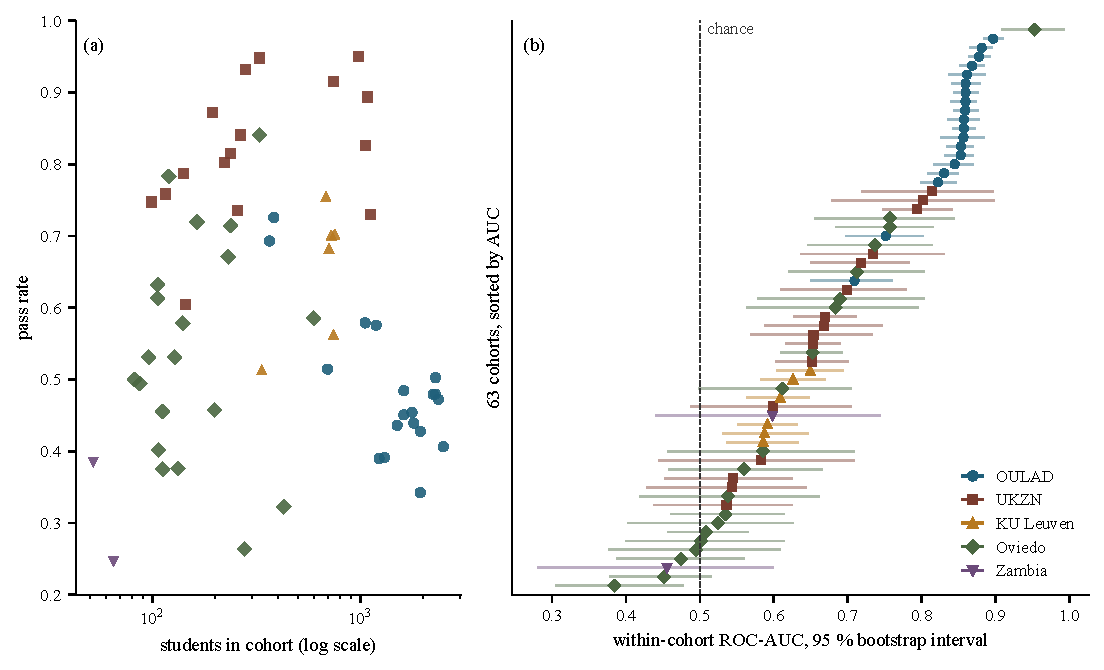
\includegraphics[width=\columnwidth]{fig2_cohort_spread.pdf}
\caption{Within-cohort ROC-AUC for every cohort, sorted, with 400-resample bootstrap intervals over students; colour marks the institution. Institution accounts for 57.3\,\% of the variance, but not cleanly: cohort size correlates 0.669 with AUC and is itself collinear with institution.}
\label{fig:spread}
\end{figure}

\subsection{Reference points, and a replication with no estimator-free answer}\label{sec:agree}

Fig.~\ref{fig:instability} places every comparison in this paper on one axis.
Two models differing only in which half of one cohort they saw agree at $\tau$ 0.338 under permutation importance. That is the most such a comparison attains under that estimator, and it is far below what a teacher-facing factor list implicitly promises. The noise floor of 0.706 confirms this is not estimator variance.

Against those bounds, the estimator comparison. Applied to one fitted model on
one set of students, permutation importance and SHAP agree at $\tau$ 0.410, permutation and drop-column at 0.259, SHAP and drop-column at 0.127. Taken bare, the two low numbers look like the conclusion of Swamy et al.\ \cite{swamy2022} --- that the explainer is a first-order determinant of the resulting factor list --- now on 63 cohorts across five institutions and three model families rather than five MOOCs and one network. Taken against the bounds, neither is a like-for-like arm: one estimator is degenerate here, and the remaining pair has no single scale.

One arm requires a caveat we report rather than hide. Four of the seven features
are cumulative counters of the same behaviour, and removing one leaves
near-duplicates behind, so drop-column importance is zero or negative for 3.2 of 7 features on average, against 2.0 for permutation and 0.1 for SHAP. Its agreement with itself across resamples of one cohort is 0.173 --- lower than its agreement with permutation on identical data, and against 0.592 for SHAP. On collinear behavioural features, drop-column is
not a reliable estimator, and 0.127 should be read as evidence about that estimator in this setting rather than as a headline. The defensible figure is the permutation-versus-SHAP agreement of 0.410, and it does not settle the question, because a cross-estimator quantity has no single estimator's scale. Against permutation importance's own within-cohort reference of 0.345 it is high, and the explainer matters \emph{less} than the training sample; against SHAP's 0.592 it is low, and the explainer matters \emph{more}, which is the ordering Swamy et al.\ report. The permutation-only ceiling of 0.338 is the strictest reference we have and supports the first reading, but it too is one estimator's. The comparison has no estimator-free answer here, and Section~\ref{sec:cond} measures why.

% Nine sentence-length category labels: at 3.4 in the tick text renders near
% 4 pt. Spanning both columns is the only way this figure stays readable.
\begin{figure*}[t]
\centering
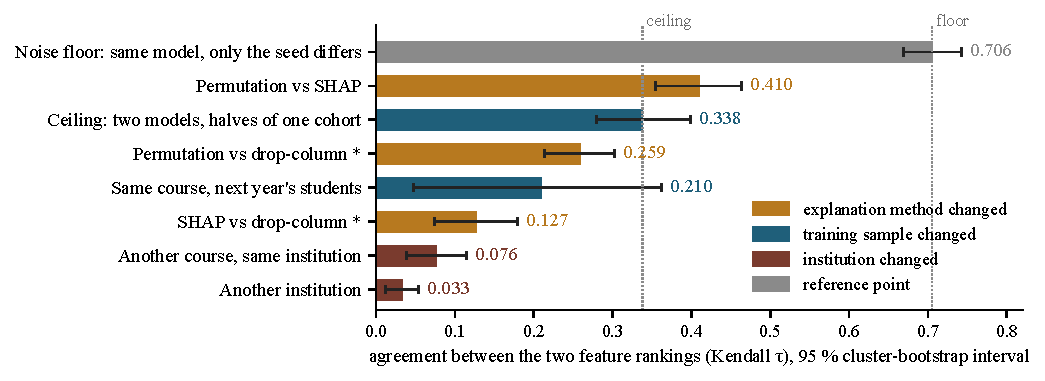
\includegraphics[width=0.70\textwidth]{fig1_explanation_instability.pdf}
\caption{Every agreement comparison in this paper on one scale, with its bounds; colour marks what differed between the two rankings. The floor and ceiling bars are measured under permutation importance and carry its scale, so a bar above them is not above a universal ceiling; each estimator's own reference is in Table~\ref{tab:cond}. Starred bars involve drop-column, degenerate here --- 3.2 of 7 features receive zero or negative importance, self-agreement 0.173.}
\label{fig:instability}
\end{figure*}

\subsection{A single-estimator study measures its own estimator}\label{sec:cond}

The practical consequence is sharper than the comparison above. Take a question the literature does ask --- how much does retraining on the next year's students change a model's feature ranking? --- and answer it three times, changing only the estimator, on the same 78 course-year pairs, the same fitted models and the same held-out thirds (Table~\ref{tab:cond}).

Each estimator needs its own reference, because they disagree on the level even when nothing is retrained. Applied twice to one cohort under two different splits, SHAP reproduces itself at $\tau$ 0.592 and permutation importance at 0.345. Against those references, a year of retraining costs 0.083 under SHAP and 0.089 under permutation: the same effect to within 0.006. The level at which that effect is reported differs by 0.252, roughly three times the effect itself. Fig.~\ref{fig:instability} shows the ladder's own D1 rung at 0.210 rather than 0.256, because the ladder scores a source model on the whole target cohort instead of a held-out third; the gap between protocols is small beside the gap between estimators.

\begin{table}[t]
\caption{The same question, three estimators, on identical models and evaluation sets: 78 course-year pairs, three splits each. The third column is the answer a study would report; the fourth is the effect it is trying to measure, differenced before rounding. $^{*}$Drop-column is degenerate here (Section~\ref{sec:agree}).}
\label{tab:cond}
\centering
\small
\begin{tabular}{@{}lccc@{}}
\toprule
Estimator & Same cohort, & Next year's & Cost of \\
 & another split & students & one year \\
\midrule
SHAP & 0.592 & 0.508 & 0.083 \\
Permutation importance & 0.345 & 0.256 & 0.089 \\
Drop-column$^{*}$ & 0.173 & 0.055 & 0.118 \\
\midrule
\multicolumn{3}{@{}l}{Spread from the estimator choice} & 0.252 \\
\multicolumn{3}{@{}l}{Effect being measured} & 0.086 \\
\bottomrule
\end{tabular}
\end{table}

A stability study that fixes one estimator therefore reports a number that is as much a property of that choice as of the data, and none we are aware of declares which estimator produced it. The recommendation is concrete and cheap: report agreement under at least two estimators, and report what each one scores when nothing has changed, since without that reference a $\tau$ has no scale.

\subsection{Three controls that changed our own conclusions}\label{sec:controls}

\textbf{A zero-training baseline.} Ranking students by cumulative active days ---
no model, no training, no labels --- reaches AUC 0.713 against 0.691 for a locally trained gradient-boosting model, beating it in 38 of 63 cohorts; logistic
regression reaches 0.717. At the Open University, on the twelve cohorts where intermediate assessment scores exist, the rule reaches 0.834 and the shared seven-feature model 0.858; adding the assessment features takes the model to 0.902.
Behavioural counters carry roughly what a single attendance counter already
carries; the value of a model here scales with what it knows beyond attendance.

\textbf{A majority-class metric.} Our first implementation computed F1 with the
default positive label, which is \emph{passing}. Every configuration looked
healthy while losing, on the class an alerting system acts upon, to a rule that
alerts everyone. The check costs one line: print the trivial rule beside every
score \cite{bosch2018}.

\textbf{Contamination.} 72 of 78 same-course pairs and 324 of 916 other-course
pairs share students between training and evaluation, up to 94\,\% of the target
cohort; cross-institution pairs are clean at under 1.5\,\%. Uncorrected,
same-course transfer appears to \emph{beat} within-cohort performance. Any
evaluation of this shape must report per-pair overlap.

\section{Discussion and Limitations}

The benchmark's value is in what it makes cheap: any group can now run a proposed model, representation or explainer against 63 cohorts from five platforms and report the same reference points we do. That is a modest contribution and a real one, since the difficulty visible in Section~\ref{sec:pred} --- results describe datasets --- has no remedy but more datasets in one place.

The measurement result is a caution rather than a discovery. Swamy et al.\ established that the explainer dominates the training sample \cite{swamy2022}; on this population that ordering holds against SHAP's reference and reverses against permutation importance's. We read that not as a refutation --- their models, features and population all differ from ours --- but as evidence that a claim of this form cannot be evaluated until the reference is named, and that naming it can decide the answer. Section~\ref{sec:cond} is the part we believe is new and the part
practitioners should act on: a stability number without a declared estimator, and without what that estimator scores when nothing has changed, is not interpretable, and the literature currently reports such numbers routinely.

\textbf{Limitations.} Seven behavioural features are strongly correlated, which
is exactly the setting in which importance is least identifiable and in which
drop-column degenerates; richer feature sets may behave differently and we cannot
test that where assessment data is unpublished. Three estimators are not
exhaustive. Outcome semantics differ across institutions and are collinear with
institution. Course calendars for three institutions are inferred rather than published. The $\tfrac{1}{3}$ cutoff is not load-bearing: at $\tfrac{1}{4}$ and $\tfrac{1}{2}$ every level moves and no ordering does, with cross-institution explanation agreement 0.038, 0.034 and 0.029 at the three cutoffs and accuracy rising with the later one. Zambia contributes two small cohorts whose intervals cover chance.
Bootstrap intervals resample pairs that share target cohorts and are narrower
than fully clustered intervals; the estimator spread in Section~\ref{sec:cond} is
reported without a significance test and rests on 78 course-year pairs, three splits each, from six course families. Everything here is correlational, and Section~\ref{sec:agree} is an
argument against reading any of these rankings causally.

\section{Conclusion}

We release a benchmark of 63 student cohorts from five universities, five
platforms and four countries, harmonised to one schema, with adapters and frozen
results. Within-cohort predictability spans 0.384 to 0.953 across those cohorts, so a single-dataset result is a statement about its dataset. We supply the floor, ceiling and random baseline an explanation-agreement number needs to be read at all, and find the reported dominance of the explainer over the training sample holds or reverses according to which estimator supplies the reference. The consequence we would most like read is narrow: a stability number reported with one estimator and no same-data reference has a level that moves by three times the effect under study when the estimator changes. Reporting two, and what each scores when nothing has changed, costs one run and makes the answer mean something.

\section*{Reproducibility}

We release the five institution adapters, the cohort definitions, the experiment code and the frozen result files, together with a script that recomputes every number in this paper from those files. We redistribute none of the student data. All five releases are published openly by their originating institutions, four of them under a DOI, and the repository records for each the source, the licence and the path an adapter expects, so the adapters read a copy the reuser downloads. \ifblind An anonymised repository is linked from the submission record; the permanent link replaces this note in the camera-ready version.\else Everything named here is at \url{https://github.com/a169n/student-risk-benchmark}.\fi

\section*{Ethics}

All five datasets are published in de-identified form by their originating institutions, and this work is a secondary analysis of those public releases: no student was contacted and no re-identification was attempted. No demographic attribute enters any model. One release ships a name column beside its hashed student identifier. We did not inspect it and cannot say whether those names are real; our adapter never reads it and joins on the hashed identifier alone. We note it so that other reusers make that choice deliberately.

\begin{thebibliography}{00}

\bibitem{kuzilek2017} J. Kuzilek, M. Hlosta, and Z. Zdrahal, ``Open University
Learning Analytics dataset,'' \emph{Sci. Data}, vol. 4, art. 170171, 2017.

\bibitem{tiukhova2026} E. Tiukhova, D. Van Landuyt, B. Baesens, and M. Snoeck,
``Open data, private learners: a de-identified student activity and performance
dataset for learning analytics,'' \emph{Sci. Data}, vol. 13, art. 548, 2026.

\bibitem{raghavjee2026} R. Raghavjee, P. R. Subramaniam, and I. Govender,
``Anonymized dataset of Information Systems and Technology students at a South
African university for learning analytics,'' \emph{Data}, vol. 11, no. 1, art. 1,
2026.

\bibitem{bettahi2025} A. Bettahi, F.-Z. Belouadha, and H. Harroud, ``A modular
and explainable machine learning pipeline for student dropout prediction in
higher education,'' \emph{Algorithms}, vol. 18, no. 10, art. 662, 2025.

\bibitem{boujmiraz2026} S. Boujmiraz, H. Darhmaoui, and A. Drissi el Maliani,
``Predicting student performance: a comprehensive review of machine learning,
deep learning, and explainable AI approaches,'' \emph{Comput. Educ.: Artif.
Intell.}, vol. 10, art. 100548, 2026.

\bibitem{guevara2025} R. Guevara-Reyes, I. Ortiz-Garc\'es, R. Andrade, F.
Cox-Riquetti, and W. Villegas-Ch, ``Machine learning models for academic
performance prediction: interpretability and application in educational
decision-making,'' \emph{Front. Educ.}, vol. 10, art. 1632315, 2025.

\bibitem{tiukhova2024} E. Tiukhova et al., ``Explainable learning analytics:
assessing the stability of student success prediction models by means of
explainable AI,'' \emph{Decis. Support Syst.}, vol. 182, art. 114229, 2024.

\bibitem{swamy2022} V. Swamy, B. Radmehr, N. Krco, M. Marras, and T. K\"aser,
``Evaluating the explainers: black-box explainable machine learning for student
success prediction in MOOCs,'' in \emph{Proc. 15th Int. Conf. Educational Data
Mining (EDM)}, 2022.

\bibitem{lopez2020} J. L\'opez-Zambrano, J. A. Lara, and C. Romero, ``Towards
portability of models for predicting students' final performance in university
courses starting from Moodle logs,'' \emph{Appl. Sci.}, vol. 10, no. 1, art. 354,
2020.

\bibitem{lopez2022} J. L\'opez-Zambrano, J. A. Lara, and C. Romero, ``Improving
the portability of predicting students' performance models by using ontologies,''
\emph{J. Comput. High. Educ.}, vol. 34, pp. 1--19, 2022.

\bibitem{gardner2023} J. Gardner, R. Yu, Q. Nguyen, C. Brooks, and R. Kizilcec,
``Cross-institutional transfer learning for educational models: implications for
model performance, fairness, and equity,'' in \emph{Proc. ACM Conf. Fairness,
Accountability, and Transparency (FAccT)}, 2023.

\bibitem{schwerter2026} J. Schwerter et al., ``Cross-course generalizability of
SRL-aligned predictive models using digital learning traces,'' arXiv:2604.22812,
2026.

\bibitem{riestra2021} M. Riestra-Gonz\'alez, M. del P. Paule-Ru\'iz, and F.
Ortin, ``Massive LMS log data analysis for the early prediction of
course-agnostic student performance,'' \emph{Comput. Educ.}, vol. 163, art.
104108, 2021.

\bibitem{jayaprakash2014} S. M. Jayaprakash, E. W. Moody, E. J. M. Laur\'ia, J.
R. Regan, and J. D. Baron, ``Early alert of academically at-risk students: an
open source analytics initiative,'' \emph{J. Learn. Anal.}, vol. 1, no. 1, pp.
6--47, 2014.

\bibitem{hooker2021} G. Hooker, L. Mentch, and S. Zhou, ``Unrestricted
permutation forces extrapolation: variable importance requires at least one more
model, or there is no free variable importance,'' \emph{Stat. Comput.}, vol. 31,
art. 82, 2021.

\bibitem{krishna2022} S. Krishna et al., ``The disagreement problem in
explainable machine learning: a practitioner's perspective,'' arXiv:2202.01602,
2022.

\bibitem{verdinelli2024} I. Verdinelli and L. Wasserman, ``Feature importance: a
closer look at Shapley values and LOCO,'' \emph{Stat. Sci.}, vol. 39, no. 4,
2024.

\bibitem{phiri2026} L. Phiri, ``A multi-source dataset for CS1 failure prediction
in a sub-Saharan African context,'' Zenodo, 2026, doi:10.5281/zenodo.21292883.

\bibitem{phiri2026paper} L. Phiri, M. Chaibela, I. Chisha, D. Pungwa,
D. Siabbaba, and B. Simukoko, ``Which CS1 students will fail? Identifying digital
markers from learning analytics in computer systems and architecture using
weighted academic momentum and interaction logs,'' arXiv:2608.16914, 2026.

\bibitem{friedman2001} J. H. Friedman, ``Greedy function approximation: a
gradient boosting machine,'' \emph{Ann. Stat.}, vol. 29, no. 5, pp. 1189--1232,
2001.

\bibitem{lundberg2017} S. M. Lundberg and S.-I. Lee, ``A unified approach to
interpreting model predictions,'' in \emph{Adv. Neural Inf. Process. Syst.
(NeurIPS)}, 2017.

\bibitem{bosch2018} N. Bosch and L. Paquette, ``Metrics for discrete student
models: chance levels, comparisons, and use cases,'' \emph{J. Learn. Anal.}, vol.
5, no. 2, pp. 86--104, 2018.

\bibitem{kritzinger2018} W. Kritzinger, M. Karner, G. Traar, J. Henjes, and W.
Sihn, ``Digital Twin in manufacturing: a categorical literature review and
classification,'' \emph{IFAC-PapersOnLine}, vol. 51, no. 11, pp. 1016--1022,
2018.

\bibitem{addanki2023} K. Addanki and L. Corrin, ``Unveiling the potential of
Digital Twin technology for Higher Education,'' in \emph{Proc. ASCILITE 2023:
People, Partnerships and Pedagogies}, ASCILITE Publications, 2023.

\bibitem{yerniyazov2026} A. Yerniyazov, B. Bakayeva, Z. Iztayev, P.
Kozhabekova, and S. Nurgaliyeva, ``A mobile system for formative assessment and
teacher-reviewed feedback,'' \emph{Int. J. Interact. Mobile Technol.}, vol. 20,
no. 15, pp. 37--50, 2026.

\end{thebibliography}

\end{document}
